\documentclass[a4paper, 11pt]{article}
\usepackage{graphicx}
\graphicspath{ {img/} }
\usepackage{amsmath}
\usepackage{pgfplots}
\usepgfplotslibrary{external}
\tikzexternalize
\pgfplotsset{width=10cm,compat=1.9}
\usepackage[pdftex]{hyperref}

% Lengths and indenting
\setlength{\textwidth}{16.5cm}
\setlength{\marginparwidth}{1.5cm}
\setlength{\parindent}{0cm}
\setlength{\parskip}{0.15cm}
\setlength{\textheight}{22cm}
\setlength{\oddsidemargin}{0cm}
\setlength{\evensidemargin}{\oddsidemargin}
\setlength{\topmargin}{0cm}
\setlength{\headheight}{0cm}
\setlength{\headsep}{0cm}

\renewcommand{\familydefault}{\sfdefault}

\title{Data Mining: Learning from Large Data Sets - Fall Semester 2015}
\author{jo@student.ethz.ch\\ umarco@student.ethz.ch\\ meiled@student.ethz.ch\\}
\date{\today}

\begin{document}
\maketitle

\section*{Approximate near-duplicate search using Locality Sensitive Hashing}
We started by closely following the techniques and algorithms described in the lecture and tutorial sessions. As required, Python 2.7 and numpy were used.
Jonathan started out by hashing each shingle with $r * b$ generated minhash functions. He then proceeded to create the signature column for that video by taking the minimum over all shingles.
In the begin, everything was done in a loop and thus very inefficient. In a next step, the code was vectorized where possible using numpy in order to make it more efficient.

Jonathan also went on to create a function which hashes the signature column and returns the bucket for each band (band size $b$). The band and according bucket as well as the video id and the shingles of that video were then emitted.

For the first submission, Marco detected candidate pairs in the reducer, calculated the Jaccard distance and classified them as duplicates if the distance was big enough. This resulted in a score of 0.79.

For submission two, he classified a candidate pair as duplicates, if they were hashed into the same buckets on six or more bands. With that approach, the achieved score was 0.88.

Daniel first restructured the data output of the mapper for simplicity with the ability to output the video id including band-hashes and shingles in a compact way. By playing around with the random number range and the modulo-factor as well as tuning the number of bands in the hash-table we got the score up to 0.98 on the training data, but just 0.89 in submission 3.

To get the score further up Daniel than tried to bring the false negatives down by classify videos as duplicates on a fairly low number of identical band-hashes, but than threw out the false positives by directly comparing all row-hashes. This did not really bring much progress, so we used the same concept, but compared the shingles directly to get the false-positives out. This lead to the semi-final submission with the score of 0.994.

For our final submission Marco set the boundary even lower to just one similar bucket (band-hashes) and prettified the shingles comparison by reuse of the the Jaccard distance function he used earlier. Final submission score: 0.997.

\maketitle

\section*{Large Scale Image Classification}
We started by closely following the techniques and algorithms described in the lecture and tutorial sessions. As required, Python 2.7, numpy as well as scikit-learn were used.
Jonathan started out again by establishing a solid code base, which allowed us to easily experiment with the given dataset. He went on to train a linear support vector machine in the mapper, then emitting the weights. On the reducer side, the mean of all emitted weights were calculated and saved. That already gave us a fair score of 0.73744.

Prof. Krause has hinted, that explicit feature mapping to higher dimensions might be useful for the project. With that in mind, we found the kernel approximation API's in scikit-learn. We have then only experimented with the RBFSampler, since other kernel approximations like Nystroem needed to be fitted to training data before doing a transformation. That, however, wouldn't work since the transform function in the mapper was used in the evaluation script.

Marco went on to further experiment with that setting by tuning hyperparameters. He also calculated the mean and standard deviation of the dataset and normalized the features in the transform function. Further experimentation included using other linear models like SGDClassifier and tuning those hyperparameters. Unfortunately, none of the experiments lead to a significantly better score.

By inspecting the scikit-learn API documentation closer, Jonathan found that AdditiveChi2Sampler can be used in combination with the RBFSampler. That gave us an immediate boost in score to over 0.81. Further tuning the hyperparameters lead to a final score of 0.83081.

Daniel could also not help to get a better score. One possibility to get better result lays in increasing the number of components of the RBFSampler, but this was not possible because we then run into a timeout.

\maketitle

\section*{Extracting Representative Elements}

Marco started out by implementing the k-means algorithm by hand, not leading to any satisfying results.

Jonathan's attempt was to use the K-Means clustering implementation from sklearn module as follows: In the first step a set of mappers create a set of cluster centers each. In the second part, all these cluster centers are reduced to the 100 cluster centers asked for in the project description. In our test environment we used 8 mappers (getting 12500 records each) and one reducer.

After some success with this method we changed to MiniBatchKMeans. This speeded up the computation, and even led to better results. We can not explain the latter.

The final issue was now to fine-tune the parameters such as size of mini-batches, and the number of clusters for the mapper and reducer. Therefore Jonathan implemented a parameter search script. It turned out that batch sizes of 700 and 700 clusters for the mapper (and of course 100 clusters for the reducer) optimized our score.

It's noteworthy that our final submission has a very high variance. The exactly same code led to our final score  of 8.60131 in the best case (submission 3722), but only to 13.17762 (sumbission 3791) in the worst case.

Daniel checked the lecture slides as well as the the web without finding any room for improvement and wrote the report.

\maketitle

\section*{Explore-Exploit tradeoffs in Recommender Systems}

We decided to go for the LinUCB Algorithm implementation as discussed on slide 38 of lecture 11.

\begin{figure}[htbp]
\begin{center}
\setlength{\fboxsep}{0pt}%
\setlength{\fboxrule}{1pt}%
\fbox{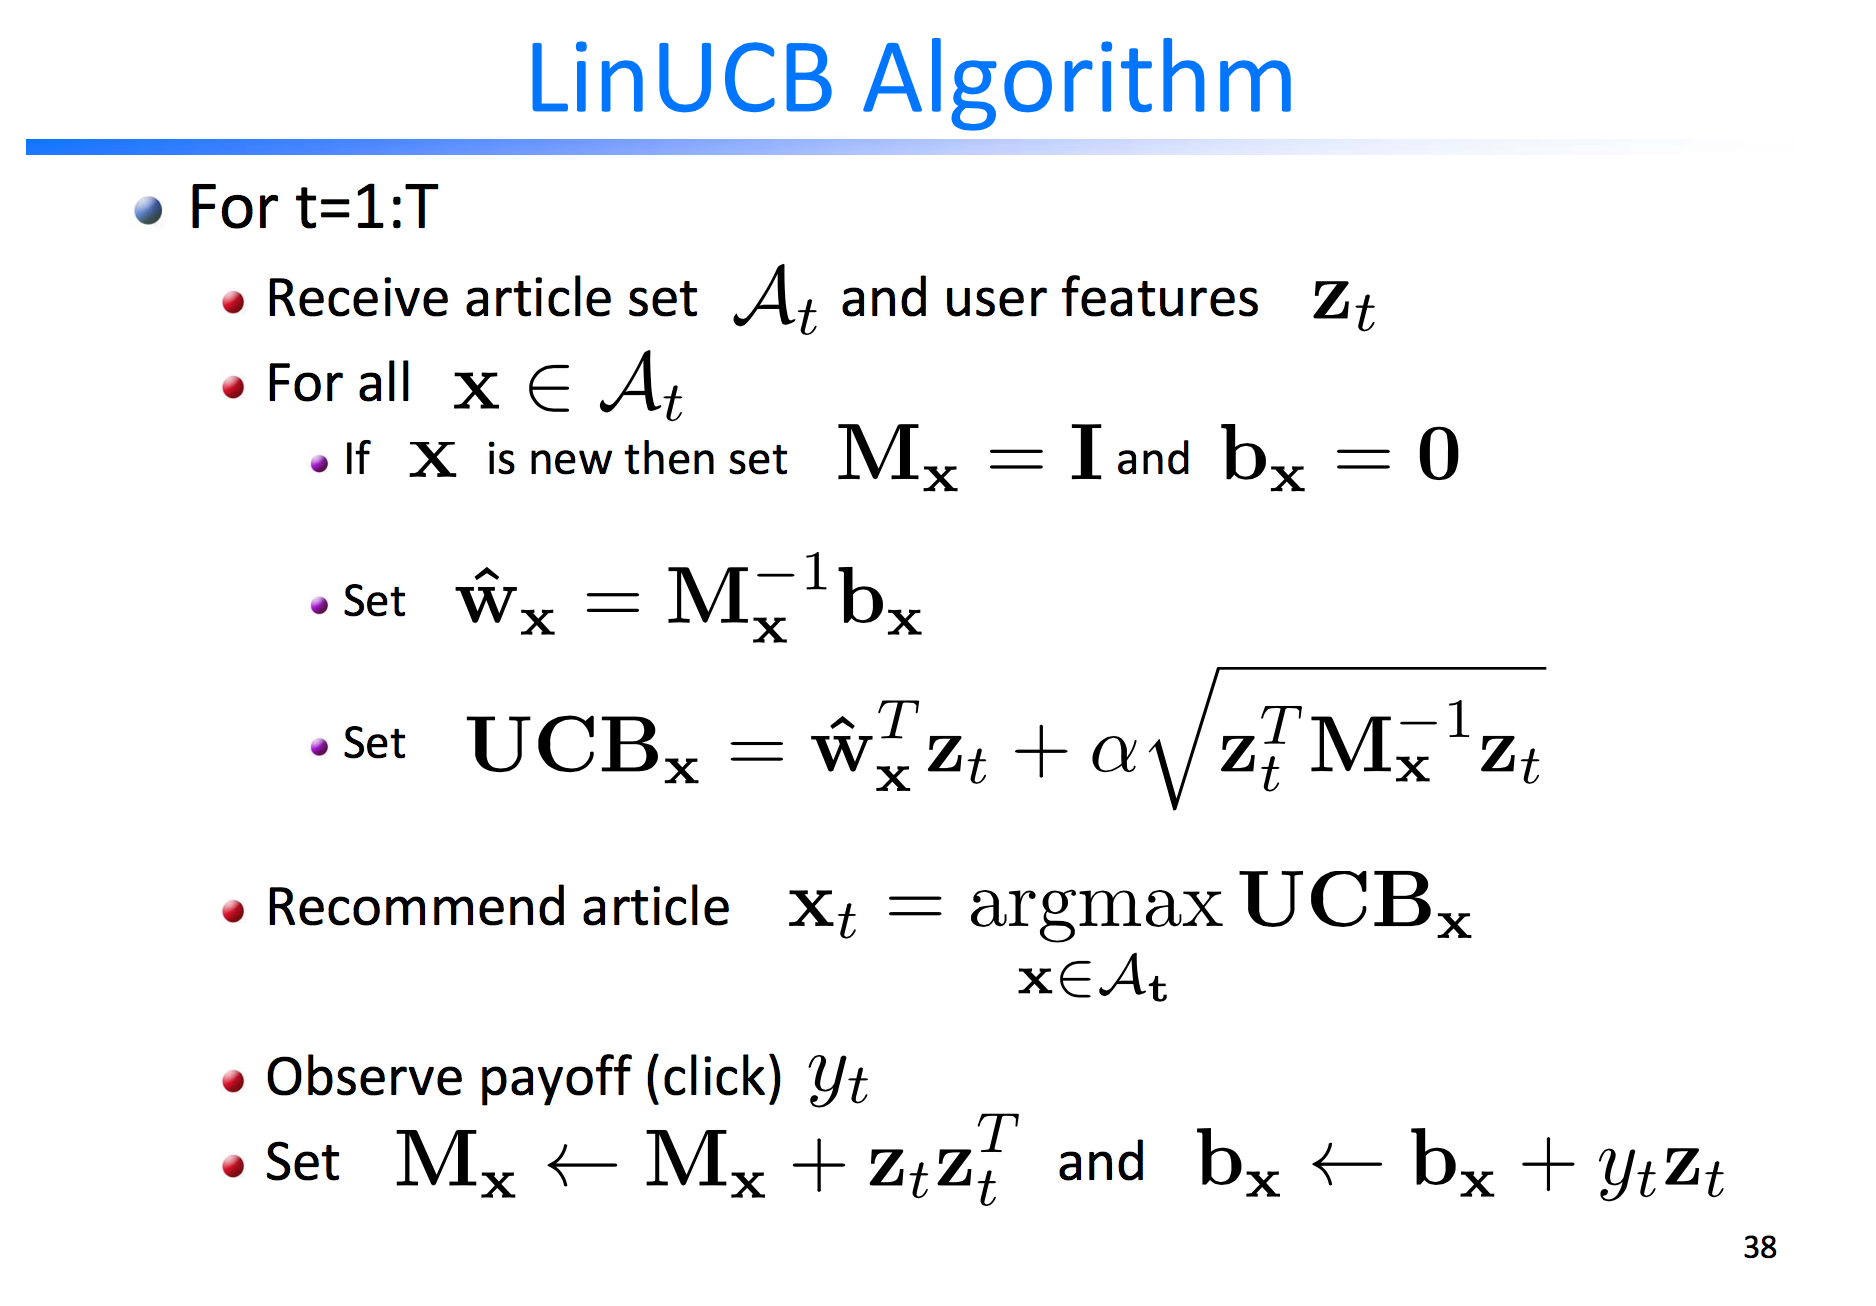
\includegraphics[width=8cm]{LinUCB_slide.png}}%

\caption{LinUCB, Slide 38 of lecture 11}
\label{default}
\end{center}
\end{figure}

Even though we're disregarding the timestamp and article features at all, we managed to get over the hard-baseline by testing different values for $\alpha$. It seems pretty random. All our submissions did run for approximately ten minutes.

\begin{figure}[htbp]
\begin{center}
\fbox{
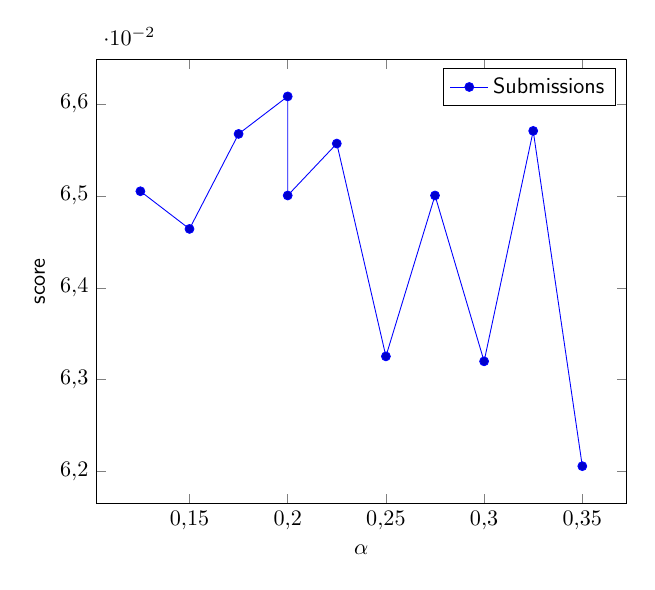
\begin{tikzpicture}[scale = 0.8]
\begin{axis}[
    /pgf/number format/.cd,
        use comma,
        1000 sep={},
        ylabel=score,
        xlabel=$\alpha$]
\addplot 
	coordinates {(0.125,0.06505)
(0.150,0.06464)
(0.175,0.065674)
(0.200,0.066082)
(0.200,0.065004)
(0.225,0.065569)
(0.250,0.063253)
(0.275,0.065004)
(0.300,0.063199)
(0.325,0.065707)
(0.350,0.062058)};

\legend{Submissions}
\end{axis}
\end{tikzpicture}

}%

\caption{Score vs. $\alpha$ in different submissions}
\label{default}
\end{center}
\end{figure}



\end{document}
